\documentclass[11pt,a4paper]{article}
\usepackage[T1]{fontenc}
\usepackage[utf8]{inputenc}
\usepackage{lmodern,microtype}
\usepackage[margin=27mm,headheight=15pt]{geometry}
\usepackage{amsmath,amssymb,amsthm,mathtools}
\usepackage{booktabs,longtable,array,enumitem}
\usepackage{graphicx,xcolor,fancyhdr}
\usepackage{xurl}
\usepackage[colorlinks=true,linkcolor=blue!45!black,citecolor=blue!45!black,urlcolor=blue!55!black]{hyperref}
\hypersetup{pdftitle={Sharp congruence bounds and finite prime sampling},pdfsubject={Two extensions of the Dirichlet-GRH proof},pdfkeywords={Dirichlet GRH, congruence modules, nonmaximal orders, central zeros, finite prime sampling}}
\newtheorem{theorem}{Theorem}[section]
\newtheorem{lemma}[theorem]{Lemma}
\newtheorem{proposition}[theorem]{Proposition}
\newtheorem{corollary}[theorem]{Corollary}
\theoremstyle{definition}
\newtheorem{definition}[theorem]{Definition}
\newtheorem{example}[theorem]{Example}
\newtheorem{remark}[theorem]{Remark}
\newcommand{\OO}{\mathcal O}
\newcommand{\Mat}{\operatorname{Mat}}
\newcommand{\GL}{\operatorname{GL}}
\newcommand{\tr}{\operatorname{tr}}
\newcommand{\len}{\operatorname{length}}
\newcommand{\Hom}{\operatorname{Hom}}
\newcommand{\Span}{\operatorname{span}}
\newcommand{\ord}{\operatorname{ord}}
\newcommand{\rank}{\operatorname{rank}}
\newcommand{\coker}{\operatorname{coker}}
\newcommand{\dd}{\,\mathrm d}
\newcommand{\code}[1]{{\small\urlstyle{tt}\nolinkurl{#1}}}
\newcommand{\srcgrh}{\href{https://github.com/lsernau/grh-lean/tree/72fead102f663d5c7a407964a13dc0cf9d977207}{\texttt{grh-lean@72fead10}}}
\newcommand{\srcarticle}{\href{https://github.com/VladimirReshetnikov/ProveIt/tree/22e5c8b7dda558fd9a50b61465483cb4c0433694/Analysis/GeneralizedRiemannHypothesis/Article}{\texttt{ProveIt@22e5c8b7}}}
\setlength{\emergencystretch}{2em}
\setlist{itemsep=3pt,topsep=5pt}
\pagestyle{fancy}
\fancyhf{}
\lhead{\small Sharp congruence bounds and finite prime sampling}
\rhead{\small 27 November 2026}
\cfoot{\thepage}
\begin{document}
\hypersetup{pageanchor=false}
\begin{titlepage}
\vspace*{12mm}
\noindent{\large\sffamily RESEARCH REPORT}\par
\vspace{8mm}
\noindent{\Huge\bfseries Sharp congruence bounds\par}
\vspace{2mm}
\noindent{\Huge\bfseries and finite prime sampling\par}
\vspace{8mm}
\noindent{\Large Two extensions of the Dirichlet-GRH proof\par}
\vspace{3mm}
\noindent{\large Prepared for Vladimir Reshetnikov\par}
\noindent{27 November 2026}
\vspace{12mm}
\begin{abstract}
We prove two results extending specific interfaces of the supplied Lean
proof of Dirichlet GRH and the accompanying ProveIt research article.
The first is unconditional: for two integral representations of dimension
$d$, trace-congruence depth $a$, and matrix-order conductor defect $e$,
the length of the intertwiner module modulo $\pi^n$ is at most
$\min(n,a)+(d^2-1)\min(n,e)$. The estimate is attained at every precision,
and it controls the coefficient primes excluded by the article's integral
Burnside assumption. A determinant-pencil argument also proves that at most
one invariant factor can exceed the defect.

The second result uses Dirichlet GRH to recover central-zero multiplicities
from a positive finite grid of prime statistics. Cascaded uniform averages,
together with local zero counts, give error
$O((\log N)^3/N^2)$ from $N$ ramp observations over logarithmic span
$O(\log N)$ for each fixed family with specified gap constants. Every fixed
grid preserves the original one-sided zero detector. We give a prescribed
schedule requiring no zero data, precise noise bounds, and an individual
complex-character version with nonnegative prime weights.
\end{abstract}
\vfill
\noindent\textbf{Evidence and scope.}
The proofs below are human-readable mathematical proofs, accompanied by
exact algebraic checks and numerical analytic diagnostics. They are not
claimed to be Lean-verified. The first theorem does not assume RH. The
second uses the supplied theorem only for Dirichlet $L$-functions.
Novelty is established relative to the inspected repository material;
global publication priority remains to be assessed.
\vspace{8mm}
\end{titlepage}
\hypersetup{pageanchor=true}
\pagenumbering{roman}
\tableofcontents
\newpage
\pagenumbering{arabic}
\section{What the sources establish and what is extended}
\label{sec:context}

\subsection{Pinned sources and the mathematical input}

The upstream source inspected here is \srcgrh, published on 25 November
2026. Its \code{grh/src/Statements.lean} imports Mathlib and states
nonvanishing for every Dirichlet $L$-function in $\Re s>1/2$, with the
principal pole excluded, as well as the corresponding critical-strip
zero statements. Its \code{Main.lean} also proves Mathlib's
\code{RiemannHypothesis}. These statements concern Dirichlet characters,
including imprimitive characters; they do not assert RH for arbitrary
automorphic or Artin $L$-functions \cite{Sernau2026}.

The repository pins Lean 4.35.0 and Mathlib commit
\code{56a005855ea17e0b0958f73ec801ae140b0a1679}.
Andrew Sutherland's independent verification report records successful
builds, axiom audits, statement comparisons and independent kernel checks
for the pinned upstream source \cite{Sutherland2026}.
The present work reads the source and those verification records; it does
not repeat the full upstream build. We use the stated Dirichlet-GRH theorem
as the analytic input of Section~\ref{grid:sec:main}.

The second source is the article at \srcarticle. Its README describes a
621-page consolidation of 103 reports and explicitly distinguishes that
consolidation from independent mathematical review \cite{ProveIt2026}.
We inspected its theorem and open-question structure, the relevant full
sections, and the three newest symplectic archives in \code{docs/incoming}.
This matters: the article's general symplectic-compression question has
already been treated in a newer incoming archive, so it is not presented
as a new contribution here.

\subsection{The source mechanism}

The upstream proof combines three inputs: a supply of short integral
forms, a spanning statement, and lower bounds forcing integral forms to
be long. In the determinant comparison, upper bounds for covolume and
index meet a lower bound obtained from twists and the product formula.
Cancellation of the common main quantity yields a one-sided estimate for
a weighted prime remainder. The meromorphic transform of that remainder
then excludes zeros to the right of the critical line. The precise entry
points are
\code{New/Reduction/MainInequality.lean},
\code{New/Reduction/OneSidedBound.lean}, and
\code{New/Reduction/Zeros/Criterion.lean} \cite{Sernau2026}.

The algebraic result below extends the global congruence term that enters
the denominator budget. The analytic result extends the subsequent
one-sided-transform and spectral-recovery interface. Thus the two results
use different parts of the supplied argument. Neither is obtained simply
by restating a standard prime-counting consequence of GRH.

\subsection{Precisely identified improvements}

\begin{longtable}{@{}p{0.24\textwidth}p{0.32\textwidth}p{0.36\textwidth}@{}}
\toprule
Interface & Inspected prior result & Result proved here\\
\midrule
Congruence modules &
\code{sel:thm:tracedepth}: length $\min(n,a)$ under full integral matrix
span; \code{sel:thm:bad}: extra torsion without it. &
The sharp bound $\min(n,a)+(d^2-1)\min(n,e)$ for nonmaximal image orders,
plus a bound on every invariant factor.\\[3pt]
Bad coefficient primes &
\code{sel:sec:open} requests an extension measured by the defect of the
image order. &
A finite conductor defect gives an explicit local and global
product-formula correction; extremal examples determine its coefficient.\\[3pt]
Finite prime sampling &
\code{ana:thm:binomial}: $(r+1)^2$ statistic samples, error
$O(\log r/\sqrt r)$, span $(1+\sqrt2)r$. &
$N$ ramp observations, error $O((\log N)^3/N^2)$, span $O(\log N)$,
with explicit dependence on fixed-family spectral constants.\\[3pt]
Central orders &
The subgroup construction recovers sums over characters, with individual
nonreal characters raised in \code{ana:q:family}. &
The real nonnegative weight $\Lambda(n)(\chi_0(n)+\Re\chi(n))$ recovers
the individual central order of $\chi$.\\
\bottomrule
\end{longtable}

The fourth entry is a simple useful corollary, not the main novelty claim.
The article also contains continuous convolution projectors and filters
using prescribed zero ordinates. The analytic advance is the finite-grid
rate, the control of all repeated aliases from a local count, and the
resulting sample and cutoff bounds. Uniform-average cascades are classical
digital filters \cite{Hogenauer1981}; no novelty is claimed for their
transfer polynomial. Likewise trace rigidity under residual absolute
irreducibility is classical \cite{Carayol1994,Brumer2019}; the new
algebraic assertion is the sharp quantitative bound without that residual
hypothesis.

Targeted searches of the literature and of the inspected sources did not
identify either exact main theorem. This is evidence for novelty relative
to the supplied program, not a proof of worldwide priority. The archive
records the search terms and the closest antecedents.

\section{A sharp congruence bound for nonmaximal image orders}
\label{order:sec:main}

\subsection{Setup and main theorem}

Let $\OO$ be a complete discrete valuation ring with fraction field $F$,
uniformizer $\pi$, and residue field $k$. Normalize $v(\pi)=1$ and set
$v(0)=\infty$. Let $G$ be an arbitrary group and
\[
 \rho,\sigma:G\longrightarrow\GL_d(\OO),\qquad d\ge1.
\]
Assume that their rational matrix spans are full:
$\Span_F\rho(G)=\Mat_d(F)=\Span_F\sigma(G)$.
The integral spans
\[
 A_\rho=\Span_{\OO}\rho(G),\qquad A_\sigma=\Span_{\OO}\sigma(G)
\]
are orders in $\Mat_d(F)$. Define
\[
 \begin{aligned}
 e_\rho&=\min\{j\ge0:\pi^j\Mat_d(\OO)\subseteq A_\rho\},\\
 e_\sigma&=\min\{j\ge0:\pi^j\Mat_d(\OO)\subseteq A_\sigma\},\qquad
 e=\min(e_\rho,e_\sigma).
 \end{aligned}
\]
Here ``conductor exponent'' means this containment exponent; it is not
an Artin conductor. Let
\[
 a=\min_{g\in G}v\bigl(\tr\rho(g)-\tr\sigma(g)\bigr),\qquad
 H_n=\{X\in\Mat_d(\OO/\pi^n):\sigma(g)X=X\rho(g)\ \forall g\in G\}.
\]
We use $\min(n,\infty)=n$. It is enough in all upper bounds below to
replace $e_\rho,e_\sigma$ by certified upper bounds and $a$ by the
valuation of any one nonzero trace discrepancy.

\begin{theorem}[Sharp trace-and-order bound]\label{thm:main}
Under these assumptions, for every integer $n\ge1$,
\begin{equation}\label{eq:main}
 \boxed{\quad \len_{\OO}H_n\le
 \min(n,a)+(d^2-1)\min(n,e).\quad}
\end{equation}
If $a<\infty$, then the rational representations are inequivalent and
\begin{equation}\label{eq:total}
 C(\rho,\sigma):=\sup_n\len_{\OO}H_n
 \le a+(d^2-1)e.
\end{equation}
Write the relation Smith exponents, including zero exponents, as
$0\le b_1\le\cdots\le b_{d^2}$, with an exponent $\infty$ for each free
summand. There is at most one infinite exponent, and
\begin{equation}\label{eq:profile}
 b_{d^2-1}\le e\quad(d\ge2),\qquad
 b_{d^2}\le a+e\quad(a<\infty).
\end{equation}
Consequently $\pi^eH_n$ is cyclic for every $n$. Both the coefficient
$d^2-1$ in \eqref{eq:total} and the loss $e$ in the last inequality of
\eqref{eq:profile} are sharp.
\end{theorem}

The statement extends the article's exact maximal-order theorem rather
than replacing it: when $e=0$ the bound becomes $\len H_n\le\min(n,a)$.
Carayol's trace-rigidity argument gives equality in that case; see also
Serre's exposition \cite[Theorem 1]{Serre1993}. For $e>0$
there need not be equality, and traces alone do not determine the module.
The defect contribution in \eqref{eq:main} stops growing once $n\ge e$.

\begin{corollary}[A scalar discrepancy]\label{cor:scalar-discrepancy}
Suppose in addition that for some $g\in G$,
$\rho(g)=\alpha I_d$ and $\sigma(g)=\beta I_d$, with $\alpha\ne\beta$.
Put $\delta=v(\alpha-\beta)$. Then, independently of possible trace
cancellation when the residue characteristic divides $d$,
\[
 \len H_n\le\min(n,\delta)+(d^2-1)\min(n,\delta,e),\qquad
 C\le\delta+(d^2-1)\min(\delta,e).
\]
These bounds are sharp for every $\delta,e\ge1$ and $d\ge2$.
\end{corollary}
\begin{proof}
The $g$ equation makes every invariant factor at most $\delta$. Combine
this with \eqref{eq:profile}. The family of Example~\ref{ex:length},
with its scalar exponent $a$ replaced by arbitrary $\delta\ge1$ without
requiring $\delta\ge e$, has Smith profile
$\delta,\min(\delta,e),\ldots,\min(\delta,e)$ and attains the bound.
The residue prime need not be prime to $d$ for this scalar statement.
\end{proof}

\subsection{Proof}

\subsubsection{Relation modules and their least exponent}

Put $m=d^2$ and $V=\Mat_d(\OO)$. For every $g\in G$ let
\[
 D_g(X)=\sigma(g)X-X\rho(g).
\]
Let $R\subseteq V^*$ be generated by all coordinate functions of all $D_g$.
Because $V^*$ is Noetherian, finitely many of these functions generate $R$.
Choose a matrix $D$ whose rows are such a finite set. Smith normal form gives
\[
 V^*/R\simeq\bigoplus_{i=1}^{m}\OO/\pi^{b_i},
\]
where a factor with $b_i=0$ is zero and a factor with $b_i=\infty$ denotes
$\OO$. In particular
\begin{equation}\label{eq:length}
 \len H_n=\sum_{i=1}^m\min(n,b_i).
\end{equation}
There is an $\OO$-basis $C_1,\ldots,C_m$ of $V$ such that every $D_g(C_i)$
has all entries in $\pi^{b_i}\OO$ when $b_i<\infty$, and vanishes when
$b_i=\infty$. For finite $b_i$ some relation has valuation exactly $b_i$.
Every basis matrix $C_i$ is primitive: some entry is a unit.

If $s=b_1<\infty$, every entry of every $D_g(X)$ is divisible by $\pi^s$
for every integral $X$. Taking $X=I_d$ gives
\begin{equation}\label{eq:mintrace}
 s\le a.
\end{equation}
If all relations are zero, full rational span forces $d=1$ and
$\rho=\sigma$, and the theorem is immediate. We henceforth exclude this
degenerate case when using $s$.

\subsubsection{The singular-intertwiner obstruction}

\begin{lemma}\label{lem:singular}
Let $X\in\Mat_d(\OO)$ be primitive and singular. If
$D_g(X)\in\pi^r\Mat_d(\OO)$ for all $g$, then $r\le e$.
The same conclusion holds after a finite extension of the valued field,
with valuations still normalized by $v(\pi)=1$.
\end{lemma}
\begin{proof}
Choose a primitive vector $v\in\OO^d$ with $Xv=0$ by clearing denominators
in a nonzero vector in the kernel over $F$. Then
$X\rho(g)v\in\pi^r\OO^d$ for every $g$, hence
$XAv\in\pi^r\OO^d$ for every $A\in A_\rho$. Choose $j$ with $v_j$ a
unit. Since $\pi^{e_\rho}E_{ij}\in A_\rho$,
\[
 \pi^{e_\rho}v_jXe_i\in\pi^r\OO^d\qquad(1\le i\le d).
\]
If $r>e_\rho$, every entry of $X$ is in the maximal ideal, contradicting
primitivity. Applying the same argument to $X^{\mathsf T}$ and the
transposed equations gives $r\le e_\sigma$. These prove $r\le e$.
Over the valuation ring of a finite extension the order containments
remain true after scalar extension, and the same argument applies.
\end{proof}

\begin{lemma}[One direction above the defect]\label{lem:pencil}
For every integer $r>e$, the image of $H_r$ under reduction to
$\Mat_d(k)$ has dimension at most one. In particular
$b_{m-1}\le e$ when $m>1$.
\end{lemma}
\begin{proof}
Suppose two classes give linearly independent residual matrices and lift
them to $X,Y\in\Mat_d(\OO)$. Every linear combination satisfies the
intertwining equations modulo $\pi^r$. Over an algebraic closure of $F$,
the homogeneous polynomial $\det(\lambda X+\mu Y)$ of degree $d>0$
has a projective zero. This is immediate if it is the zero polynomial;
otherwise every positive-degree homogeneous polynomial in two variables
has a zero in the projective line. The zero is defined over a finite
extension. Normalize its coordinates so that $\lambda,\mu$ are integral
and at least one is a unit. Independence of the residual matrices survives
residue-field extension, so $Z=\lambda X+\mu Y$ is primitive. It is
singular and intertwines modulo $\pi^r$, contradicting
Lemma~\ref{lem:singular}. In Smith coordinates the indicated image has
dimension exactly $\#\{i:b_i\ge r\}$. Take $r=e+1$.
\end{proof}

The pencil argument is why the result concerns absolute matrix span.
Over a residue field without extension, a two-dimensional pencil can
avoid singular matrices at all rational projective points. Passing to a
finite extension is essential and is permitted because the order
containment remains valid there.

\subsubsection{The longest direction and the missing unit of loss}

Assume first that $a<\infty$. A nonzero rational intertwiner between
two absolutely irreducible representations of equal dimension is an
isomorphism, which would force equal traces. Thus the rational Hom space
vanishes and all $b_i$ are finite. Write $b=b_m$ and choose the primitive
Smith basis matrix $X=C_m$. If $b\le e$, then \eqref{eq:mintrace} and
\eqref{eq:length} already give
\[
 C=\sum_i b_i\le a+(m-1)e.
\]

Suppose now $b>e$. Lemma~\ref{lem:singular} shows that $X$ is invertible
over $F$. Let
$0=t_1\le\cdots\le t_d=t$ be its matrix Smith exponents; the first is
zero because $X$ is primitive. If $t>0$, use integral invertible row and
column operations to write $X=P\operatorname{diag}(\pi^{t_i})Q$, with
unit factors absorbed into $P,Q$, and set
\[
 Y=P E_{dd}Q,\qquad Z=X-\pi^tY.
\]
The matrix $Z$ is singular and remains primitive: the zero Smith exponent
occurs in a different position because $t>0$. Since every relation on
every integral matrix is divisible by $\pi^s$,
\[
 D_g(Z)\in\pi^{\min(b,t+s)}\Mat_d(\OO)\qquad(g\in G).
\]
Lemma~\ref{lem:singular} and $b>e$ therefore imply
\begin{equation}\label{eq:compensation}
 t+s\le e.
\end{equation}
This also proves $t\le e$. If $t=0$, that inequality is immediate and
the extra compensation is unnecessary.

Now $X^{-1}\in\pi^{-t}\Mat_d(\OO)$, and
\[
 \sigma(g)-X\rho(g)X^{-1}=D_g(X)X^{-1}
 \in\pi^{b-t}\Mat_d(\OO).
\]
Taking traces yields
\begin{equation}\label{eq:trace-long}
 b\le a+t\le a+e.
\end{equation}
If $t=0$, Lemma~\ref{lem:pencil} gives
$C\le b+(m-1)e\le a+(m-1)e$.
If $t>0$, then $m>1$ and
\[
 C\le b+s+(m-2)e
 \le (a+t)+(e-t)+(m-2)e
 =a+(m-1)e.
\]
Thus the order loss that can enlarge the longest invariant factor is
paid back by a smaller shortest factor. Bounding the factors separately
would lose one unnecessary copy of $e$.

For $a=\infty$, Lemma~\ref{lem:pencil} still bounds all but one
exponent by $e$, including the assertion that there is at most one free
factor. It gives $\len H_n\le n+(m-1)\min(n,e)$ directly.

Finally let $a<\infty$ and fix $n$. If $n\le e$, use $s\le a$ to get
$\len H_n\le\min(n,a)+(m-1)n$. If $n>e$ and $a\ge n$, use
Lemma~\ref{lem:pencil}. If $n>e$ and $a<n$, use the total bound just
proved. This establishes \eqref{eq:main} in every case. The cyclicity of
$\pi^eH_n$ follows from the Smith profile. This completes the proof of
the bounds in Theorem~\ref{thm:main}.

\subsection{Sharpness and exact examples}

\subsubsection{The exponent loss is necessary}

\begin{example}\label{ex:exponent}
Let $\OO=\mathbb Z_p$, let $a,e\ge1$, and let $G$ be free on $u,v,z$.
Set
\[
\begin{array}{lll}
 \rho(u)=I+p^eE_{12},&\rho(v)=I+E_{21},&\rho(z)=I,\\
 \sigma(u)=I+E_{12},&\sigma(v)=I+p^eE_{21},&
 \sigma(z)=\operatorname{diag}(1,1+p^a).
\end{array}
\]
Both image-order conductor exponents equal $e$. The $u,v$ equations force
\[
 X=\operatorname{diag}(x,p^ex)
\]
over every quotient ring, with no additional torsion coordinates. The
$z$ equation is $p^{a+e}x=0$. Consequently the relation Smith exponents are
$(0,0,0,a+e)$, and
\[
 \len H_n=\min(n,a+e).
\]
The trace depth is $a$. Indeed, conjugation of $\rho$ by
$\operatorname{diag}(1,p^e)$ agrees with $\sigma$ on $u,v$ and agrees
modulo $p^a$ on $z$. These conjugated matrices are integral, so their
traces agree modulo $p^a$ on every word and its inverse. The trace
discrepancy at $z$ is $-p^a$.

For the order assertions, $A_\rho$ has basis
$I,E_{21},p^eE_{12},p^eE_{11}$. The analogous order for $\sigma$ has basis
$I,E_{12},p^eE_{21},p^{\min(a,e)}E_{11}$. They are closed under
multiplication, contain the generators and their inverses, and are
generated by their indicated differences and products. The off-diagonal
condition proves that their conductor exponent is exactly $e$.
\end{example}

\subsubsection{The length coefficient is necessary}

\begin{example}\label{ex:length}
Let $d\ge2$, choose a prime $p\nmid d$, and take $a\ge e\ge1$. Let $G$
be free on $z$ and $x_{ij}$, $1\le i,j\le d$. Put
\[
 \rho(x_{ij})=\sigma(x_{ij})=I+p^eE_{ij},\quad
 \rho(z)=I,\quad\sigma(z)=(1+p^a)I.
\]
Every generator is invertible over $\mathbb Z_p$. Both image orders are
$\OO I+p^e\Mat_d(\OO)$, with conductor exponent $e$. The centralizer
relations have one zero Smith factor and $d^2-1$ factors $p^e$:
commuting with every matrix unit means precisely that all off-diagonal
entries vanish and all diagonal entries are equal. The scalar $z$
relation therefore gives
\[
 (b_1,\ldots,b_{d^2})=(e,\ldots,e,a),\qquad
 \len H_n=\min(n,a)+(d^2-1)\min(n,e).
\]
The trace discrepancy at $z$ is $-dp^a$, of valuation $a$; all
discrepancies are divisible by $p^a$. This proves equality in the main
bound and the optimality of its coefficient $d^2-1$.
\end{example}

\subsubsection{The complete defect profile for scalar twists}

\begin{proposition}\label{prop:scalar}
Let $\tau:J\to\GL_d(\OO)$ have full rational span, and let the
commutator relation module for $\tau$ have invariant decomposition
\[
 Q_{\rm ad}\simeq\OO\oplus\bigoplus_{i=1}^{d^2-1}\OO/\pi^{c_i},
 \qquad c_i\ge0.
\]
Let $u\in\OO^\times$, $u\ne1$, and put $b=v(u-1)$. On
$G=J\times\mathbb Z$ define
\[
 \rho(h,r)=\tau(h),\qquad\sigma(h,r)=u^r\tau(h).
\]
If $t$ is the valuation of the ideal generated by
$\{\tr\tau(h):h\in J\}$, then the trace depth is $a=b+t$ and
\[
 \len H_n=\min(n,b)+\sum_i\min(n,b,c_i),\qquad
 C=b+\sum_i\min(b,c_i).
\]
In particular this is an exact bad-order replacement for trace depth,
with the full centralizer-defect profile retained.
\end{proposition}
\begin{proof}
The equations for $J$ are commutation with $\tau$, and the equation for
the generator of $\mathbb Z$ is $(u-1)X=0$. Thus $H_n$ is the
$\pi^b$-torsion of the finite-level commutant. Apply its Smith formula.
Every trace discrepancy is $(1-u^r)\tr\tau(h)$; the ideal generated by
$1-u^r$ for integers $r$ is $(1-u)$, since $r=1$ occurs and the geometric
sum works also for negative $r$ using the unit $u$. This proves $a=b+t$.
The trace ideal is nonzero because the matrix span is full and the trace
map on $\Mat_d(F)$ is nonzero in every characteristic.
\end{proof}

\subsection{Finite certificates and arithmetic consequences}

\subsubsection{What a finite computation certifies}

If $G$ is generated by a finite set $S$, the intertwining equations for
$S$ already imply the equations for every group element over every
quotient ring. For products use
\[
 D_{gh}(X)=\sigma(g)D_h(X)+D_g(X)\rho(h),
\]
and for inverses use
$D_{g^{-1}}(X)=-\sigma(g)^{-1}D_g(X)\rho(g)^{-1}$.
Hence a Smith form of the stacked generator equations computes the exact
module, with no enumeration of long words. This requires generators of
the joint image of $(\rho,\sigma)$; generators of just one image are
insufficient.

To certify an upper bound $e_\rho$, choose finitely many words whose
matrices span a lattice $L\subseteq A_\rho$ of full rank in
$\Mat_d(\OO)$. The largest Smith exponent of the coordinate matrix for
$L$ is an upper bound for $e_\rho$. The same applies to $\sigma$.
Any exact trace discrepancy provides an upper bound for $a$. Substituting
these three certified quantities into Theorem~\ref{thm:main} is sound,
even if the finite matrix samples do not generate the whole image order
and even if the trace sample does not attain the minimum.

When entries admit exact arithmetic, a complete image-order basis can be
computed by starting with $\OO I$ and adjoining products by the generator
matrices and their inverses until the module stabilizes. Noetherianity
ensures termination. A stable module is the whole order because it
contains the identity and is stable under all generator words. This is
an algebraic algorithm for an explicitly presented joint image, not a
claim that arbitrary Galois images can be determined effectively.

\subsubsection{The conjugate-dual term of the supplied article}

For the article's pair $\sigma=D(\rho)$, inversion and conjugation
permute group elements, transposition preserves the full matrix lattice,
and multiplying individual group matrices by units leaves their span
unchanged. Thus the two conductor exponents coincide. With that common
value $e$, a nonzero trace discrepancy of valuation $a$ certifies
\[
 C(T)\le a+(d^2-1)e.
\]
More accurately, use the minimum trace depth if it is known. This
quantifies the bad coefficient-prime correction that the article leaves
open. It does not remove the integral matrix-span hypothesis from every
other use in the source: local cocycle ranks, scalar inertia, and the
automorphic twisting construction still need their own arguments.
If the source's scalar element is available with discrepancy depth
$\delta$, Corollary~\ref{cor:scalar-discrepancy} instead gives
$C(T)\le\delta+(d^2-1)\min(\delta,e)$, recovering the full-span
cyclic bound at $e=0$ without tracing a scalar matrix.

For a compatible system over a number field $L$, suppose a fixed
nonzero ideal $J$ is generated by exact common trace discrepancies and
the local orders have certified conductor exponents $e_\lambda$. At all
places where the hypotheses hold,
\[
 C_\lambda\le v_\lambda(J)+(d^2-1)e_\lambda.
\]
If only finitely many $e_\lambda$ are nonzero, put
$\mathfrak f=\prod_\lambda\lambda^{e_\lambda}$, excluding any designated
places as necessary. Then
\[
 \sum_\lambda C_\lambda\log N\lambda
 \le\log N(J)+(d^2-1)\log N(\mathfrak f).
\]
This is exactly the additive form needed for the source's product-formula
budget, with a separately visible correction at bad coefficient primes.


% Research draft prepared for the parent agent. Standalone mathematical content.
% Standard packages: amsmath, amssymb, amsthm. No nonstandard macros needed.
\section{Finite positive grids isolate central zeros}
\label{grid:sec:main}

The construction below uses the classical cascade of finite uniform averages
(the normalized transfer polynomial of a cascaded integrator--comb filter~\cite{Hogenauer1981}).
The contribution is the quantitative arithmetic application: unit-interval
zero counts control its repeated high-frequency aliases, so a finite positive
grid attains nearly quadratic accuracy in its number of samples while
preserving the one-sided zero-detection argument.

\subsection{An explicit averaging lemma}

For integers $k\ge2$, $m\ge1$, define
\[
 U_k(w)=\frac1{k+1}\sum_{j=0}^{k}e^{jw/k},\qquad
 \mathcal A_{k,m}f(t)=\sum_{j=0}^{mk}p_j f(t+j/k),
\]
\[
 \sum_{j=0}^{mk}p_jz^j=\left(\frac{1+z+\cdots+z^k}{k+1}\right)^m.
\]
All $p_j$ are positive rationals and $\sum p_j=1$. The operator has $mk+1$
distinct taps and support length $m$. Its multiplier on $e^{wt}$ is $U_k(w)^m$.

\begin{lemma}[Uniform contraction away from the aliases]\label{grid:lem:contraction}
For $0<\theta\le\pi$, $k\ge2$, and
$\operatorname{dist}(\gamma,2\pi k\mathbb Z)\ge\theta$,
\[
 |U_k(i\gamma)|\le\exp\left(-\frac{\theta^2}{6\pi^2}\right).
\]
For $a>0$,
\[
 0<U_k(-a)\le v_a:=\frac{1+e^{-a}}2<1.
\]
\end{lemma}
\begin{proof}
Reduce $\gamma$ modulo $2\pi k$ to $\delta\in[-\pi k,\pi k]$.
If $|\delta|\le\pi$, let $X,Y$ be independent and uniform on
$\{0,1/k,\ldots,1\}$. Then
\[
 1-|U_k(i\delta)|^2
 =\mathbb E[1-\cos(\delta(X-Y))]
 \ge\frac{2\delta^2}{\pi^2}\mathbb E(X-Y)^2
 =\frac{k+2}{3k\pi^2}\delta^2\ge\frac{\delta^2}{3\pi^2}.
\]
Here $1-\cos u\ge2u^2/\pi^2$ for $|u|\le\pi$, and
$\operatorname{Var}X=(k+2)/(12k)$. Thus
$|U_k(i\delta)|\le e^{-\delta^2/(6\pi^2)}$.
If $\pi\le|\delta|\le\pi k$, the geometric-sum formula gives
\[
 |U_k(i\delta)|\le\frac1{(k+1)\sin(|\delta|/(2k))}
 \le\frac1{(k+1)\sin(\pi/(2k))}\le\frac1{\sqrt2}.
\]
The last inequality follows from concavity of sine on $[0,\pi/4]$:
$\sin x\ge(2\sqrt2/\pi)x$ there. Since $2^{-1/2}<e^{-1/6}$,
this also gives the asserted bound. Finally convexity puts $e^{-ax}$ below
its endpoint chord on $[0,1]$; averaging at mean $1/2$ proves the second claim.
\end{proof}

\begin{theorem}[Alias-controlled positive spectral projection]\label{grid:thm:abstract}
Let $\Gamma\subset\mathbb R\setminus\{0\}$ be locally finite, with
$|\gamma|\ge\eta>0$, nonnegative masses $\nu_\gamma$, and constants $A,B,E,a>0$.
Suppose
\[
 \sum_{\gamma\in\Gamma\cap[u-\pi,u+\pi]}\nu_\gamma
 \le A\log(2+|u|)\quad(u\in\mathbb R),\qquad
 |c_\gamma|\le\frac{B\nu_\gamma}{1/4+\gamma^2},
\]
and
\[
 f(t)=c_0+\sum_{\gamma\in\Gamma}c_\gamma e^{i\gamma t}+E_0(t),
 \qquad |E_0(t)|\le E e^{-at}\quad(t\ge0).
\]
Set $W=\sum_{\gamma\in\Gamma}\nu_\gamma/(1/4+\gamma^2)$,
$\theta=\min(\pi,\eta)$,
$\kappa=\min\{\theta^2/(6\pi^2),-\log v_a\}>0$, and $C_*=2+2\pi$.
Then $W<\infty$, and for all $k\ge2$, $m\ge1$, $t\ge0$,
\begin{equation}\label{grid:eq:bound}
 |\mathcal A_{k,m}f(t)-c_0|
 \le BW e^{-\theta^2m/(6\pi^2)}+Ee^{-at}v_a^m
 +\frac{2AB}{\pi^2 k^2}
 \left\{\zeta(2)\log(C_*k)-\zeta'(2)\right\}.
\end{equation}
In particular, with $m_k=\lceil2\log k/\kappa\rceil$,
\[
 \sup_{t\ge0}|\mathcal A_{k,m_k}f(t)-c_0|
 \le\frac{BW+E+(2AB/\pi^2)
 [\zeta(2)\log(C_*k)-\zeta'(2)]}{k^2}.
\]
\end{theorem}
\begin{proof}
The local count implies absolute summability by summing
$O(\log(2+|n|)/(1+n^2))$ over unit intervals. Hence averaging the series
term by term is legitimate, uniformly in $t$. Away from the intervals
$I_\ell=(2\pi k\ell-\theta,2\pi k\ell+\theta)$, the preceding lemma
gives the first term in \eqref{grid:eq:bound}. The interval $I_0$ contains no
frequency, since $\theta\le\eta$. For $\ell\ne0$ and $\gamma\in I_\ell$,
$|\gamma|\ge\pi k|\ell|$; the local count and $|U_k(i\gamma)|\le1$ give
\[
 \sum_{\gamma\in I_\ell}|c_\gamma|\,|U_k(i\gamma)|^m
 \le\frac{AB\log(2+2\pi k|\ell|)}{\pi^2 k^2\ell^2}.
\]
Use $2+2\pi k\ell\le C_*k\ell$ for $\ell\ge1$ and sum over both
signs of $\ell$. The two elementary sums are
$\sum\ell^{-2}=\zeta(2)$ and
$\sum(\log\ell)/\ell^2=-\zeta'(2)$.
The averaged remainder is at most $Ee^{-at}U_k(-a)^m$.
The choice of $m_k$ makes both exponential factors at most $k^{-2}$.
\end{proof}

The same proof gives $O(e^{-\kappa m}+\log k/k^r)$ for
$|c_\gamma|\le B\nu_\gamma(1+|\gamma|)^{-r}$, $r>1$;
the alias constant uses $\zeta(r)$ and $-\zeta'(r)$. Choosing
$m\ge(r/\kappa)\log k$ with $m\asymp\log k$, the error in
$N\asymp k\log k$ taps is
$O((\log N)^{r+1}/N^r)$.

\begin{proposition}[The alias term cannot be removed from this information class]
For every integer $k\ge2$, any probability measure supported on
$k^{-1}\mathbb Z$ has Fourier transform equal to $1$ at $2\pi k$.
There are symmetric spectra obeying the count and gap hypotheses above,
with constants independent of $k$, for which the error of every such
averaging rule at $t=0$ is at least $c\log k/k^2$.
\end{proposition}
\begin{proof}
Put mass $M_k=\lfloor\log(2+2\pi k)\rfloor$ at each of
$\gamma=\pm2\pi k$, use coefficients
$M_k/(1/4+(2\pi k)^2)$, and set $E_0=0$. These spectra satisfy the
local count with one absolute constant, and have a fixed positive gap.
Every lattice sample sees both exponentials as $1$, so every probability
average leaves their total $2M_k/(1/4+4\pi^2k^2)$ unchanged.
This is a lower bound for the abstract spectral class, not a claim that
Dirichlet zero ordinates equal these aliases.
\end{proof}

\subsection{Prime statistics with positive spectral weights}

Let $\mathcal C$ be a finite multiset of Dirichlet characters, with positive
real weights $b_\chi$, invariant under conjugation. Put
\[
 a(n)=\Lambda(n)\sum_{\chi\in\mathcal C}b_\chi\chi(n),\quad
 S(x)=\sum_{n\le x}a(n)\left(\frac1n-\frac1x\right),\quad
 \delta=\sum_{\chi\text{ principal}}b_\chi,
\]
and define, directly from prime powers and with no centering constant,
\[
 d(t)=\frac{e^{(t+1)/2}}{e^{1/2}-1}
 \{\delta+S(e^t)-S(e^{t+1})\},\qquad
 M=\sum_\chi b_\chi\operatorname{ord}_{s=1/2}L(s,\chi).
\]
Imprimitive Euler factors are nonzero at $1/2$ and are absorbed into the
decaying remainder. Under Dirichlet GRH, the ramp explicit formula gives
\begin{equation}\label{grid:eq:prime-expansion}
 d(t)=4M+\sum_{\gamma\ne0}
 \frac{K(i\gamma)\nu_\gamma}{1/4+\gamma^2}e^{i\gamma t}
 +O_{\mathcal C}(e^{-t/4}),\qquad
 K(w)=\frac{e^{1/2}-e^w}{e^{1/2}-1},
\end{equation}
where $\nu_\gamma=\sum_\chi b_\chi\operatorname{ord}_{1/2+i\gamma}L(s,\chi^*)$.
The standard local zero count supplies $A$, discreteness supplies $\eta>0$,
and $|K(i\gamma)|\le B=(e^{1/2}+1)/(e^{1/2}-1)$. Formula
\eqref{grid:eq:prime-expansion} follows by applying
$(e^{1/2}I-T_1)/(e^{1/2}-1)$ to the centered normalized ramp; the constant
in the centered ramp cancels exactly in the displayed definition of $d$.

Here are the analytic details behind this input. Set
$D(s)=-\sum_\chi b_\chi L'(s,\chi)/L(s,\chi)$ and write
$D(s)=\delta/(s-1)+d_0+O(s-1)$ near $1$. For $\Re s>1$, integrating
each ramp term gives
\[
 \int_1^\infty S(x)x^{-s}\dd x=\frac{D(s)}{s(s-1)}.
\]
Thus, with $c=d_0-\delta$ and $R(x)=S(x)-\delta\log x-c$,
\[
 \Phi(s):=\int_1^\infty R(x)x^{-s}\dd x
 =\frac{D(s)}{s(s-1)}-\frac{\delta}{(s-1)^2}-\frac c{s-1}.
\]
The apparent pole at $1$ is removable. At a nontrivial zero $\rho$ its
residue is $\nu_\rho/(\rho(1-\rho))$, where the weighted multiplicity
$\nu_\rho$ is positive. Under Dirichlet GRH, Mellin inversion for the
continuous ramp and a contour shift to $\Re s=1/4$ therefore give
\[
 R(x)=\sum_\gamma
 \frac{\nu_\gamma x^{-1/2+i\gamma}}{1/4+\gamma^2}
 +O_{\mathcal C}(x^{-3/4}).
\]
The integral on the new vertical line converges absolutely: the
logarithmic derivatives are $O_{\mathcal C}(\log(2+|\Im s|))$ there,
by the usual partial-fraction expression and local zero counts, and
the denominator has quadratic decay. Horizontal edges are taken at
heights avoiding the zeros; the bound $O_{\mathcal C}(\log^2 T)$ for
the logarithmic derivatives there makes their integrals tend to zero.
Finite Euler factors have no zero in $\Re s>0$, so create no residue
in this shift. Local zero counts, including multiplicities, can be
taken from \cite{Bennett2021}; the analogous zeta estimate is also
part of the upstream analytic development. This proves the claimed
uniform remainder after multiplying by $\sqrt x$ and applying $K$.
The cancellation of $c$ is exact, so its value is never an input to
the statistic.

\begin{theorem}[Central multiplicity from a finite grid]\label{grid:thm:prime}
For the fixed family $\mathcal C$, let $m_k$ be as in
Theorem~\ref{grid:thm:abstract}, and set
\[
 Z_k(t)=\tfrac14\mathcal A_{k,m_k}d(t),\qquad
 N_k=(m_k+1)k+1.
\]
Then uniformly for $t\ge0$,
\[
 Z_k(t)=M+O_{\mathcal C}(\log k/k^2)
       =M+O_{\mathcal C}((\log N_k)^3/N_k^2).
\]
The statistic uses exactly the grid of $N_k$ ramp values
$S(e^{t+j/k})$, $0\le j\le(m_k+1)k$. At $t=0$ it uses prime powers only
up to $e^{m_k+1}=N_k^{O_{\mathcal C}(1)}$, and its logarithmic span is
$m_k+1=O_{\mathcal C}(\log N_k)$. If $M$ is an integer, rounding $Z_k(t)$
to the nearest integer is valid once the explicit right side of
\eqref{grid:eq:bound}, divided by $4$, is below $1/2$.
\end{theorem}

If no spectral gap is provided, a completely prescribed choice
$m_k=\lceil\log k\,\log\log(k+e^e)\rceil$ eventually makes the exponential
terms at most $k^{-2}$ for every fixed family. It gives
\[
 Z_k(t)-M=O_{\mathcal C}
 \left(\frac{(\log N_k)^3(\log\log N_k)^2}{N_k^2}\right),
 \qquad e^{m_k+1}=N_k^{O(\log\log N_k)}.
\]
The onset is family-dependent. Neither version claims uniformity in
unbounded conductor or a practical cutoff without explicit $A,E,\eta$.

\subsection{Noise, individual characters, and the one-sided converse}

If each observed $d$ value has error at most $\epsilon$, positivity and
$\sum p_j=1$ give error at most $\epsilon/4$ in $Z_k$. Alternatively,
if the normalized ramp values
$Y_j=e^{(t+j/k)/2}S(e^{t+j/k})$ have error at most $\epsilon$, then
\[
 |Z_k^{\rm obs}-Z_k|\le\frac B4\epsilon.
\]
Indeed
$d(t+j/k)=[e^{1/2}Y_j-Y_{j+k}+\delta e^{(t+j/k+1)/2}]/(e^{1/2}-1)$.
No bound independent of the span is claimed for uniform absolute error
in the unnormalized $S$ values. Those errors are multiplied by
the displayed exponential factors.

For any nonprincipal character $\chi$ modulo $q$, a single real
nonnegative arithmetic weight suffices for its individual central order:
\[
 a_\chi(n)=\Lambda(n)\{\chi_0(n)+\operatorname{Re}\chi(n)\}\ge0.
\]
It corresponds to weights $1,1/2,1/2$ on $\chi_0,\chi,\bar\chi$;
repeated characters are combined. Since conjugation gives equal central
orders and the principal $L$-function has no zero at $1/2$, its $M$ is
exactly $\operatorname{ord}_{1/2}L(s,\chi)\in\mathbb Z_{\ge0}$.
For completeness, $\zeta(1/2)=\eta(1/2)/(1-\sqrt2)<0$, since the
alternating eta series at $1/2$ is positive; the finitely many omitted
Euler factors of a principal character are nonzero at $1/2$.
For noncentral zeros the same statistic detects all three factors.
Thus no assumption about central nonvanishing, simple zeros, separation
between distinct noncentral ordinates, or rational independence is used.

\begin{lemma}[One-sided meromorphic Laplace principle]\label{grid:lem:landau}
Let a real continuous function $f$ on $[0,\infty)$ have at most
exponential growth, and suppose its Laplace transform admits a
meromorphic continuation to $\Re w>0$. Suppose every pole on the
positive real axis is simple with positive residue. If
$f(t)\le C e^{\sigma t}$ eventually, where $\sigma\ge0$, then that
continuation has no pole in $\Re w>\sigma$.
\end{lemma}
\begin{proof}
Choose $T$ beyond which $g(t)=Ce^{\sigma t}-f(t)\ge0$, and put
$g(t)=0$ for $t<T$. Its Laplace transform has a finite convergence
abscissa $\alpha$, unless it converges everywhere, in which case the
claim is immediate. A Laplace transform of a nonnegative function
must be singular at its finite real convergence abscissa. Indeed,
if it were holomorphic there, its Taylor expansion at a real point
$u>\alpha$ close to $\alpha$, evaluated to the left of $u$, has
nonnegative terms
$\int_T^\infty t^j g(t)e^{-ut}\dd t\,(u-v)^j/j!$.
Holomorphy and monotone convergence would then imply convergence
at some $v<\alpha$, a contradiction. This is Landau's positivity
argument, also used in the supplied proof.

If $\alpha>\sigma$, the meromorphic identity for this transform
is $C e^{-(w-\sigma)T}/(w-\sigma)$ minus the transform of $f$,
up to an entire initial-interval term. At the required singularity
$w=\alpha$ it would therefore have a simple pole with negative
residue. Its values would tend to $-\infty$ as $w\downarrow\alpha$,
contrary to nonnegativity of its defining integral. Hence
$\alpha\le\sigma$. Its integral is holomorphic in $\Re w>\sigma$,
and the same meromorphic identity shows the asserted absence of
poles for the transform of $f$.
\end{proof}

\begin{theorem}[Every fixed grid retains one-sided zero detection]
Fix $k\ge2$ and $m\ge1$. For the conjugation-invariant positive-weight
family above, GRH for all its factors is equivalent to an eventual upper
bound on $\mathcal A_{k,m}d(t)$, and to an eventual two-sided bound.
If one of the factors has a zero $\rho$ with
$\operatorname{Re}\rho>1/2+\sigma$, $\sigma\ge0$, then
\[
 \limsup_{t\to\infty}e^{-\sigma t}\mathcal A_{k,m}d(t)=+\infty.
\]
\end{theorem}
\begin{proof}
The shifted Laplace transform of the centered ramp has, at
$w=\rho-1/2$, residue $\nu_\rho/(\rho(1-\rho))$. Taking a finite forward
shift multiplies its meromorphic continuation by $e^{hw}$ up to an entire
function (the contribution of the initial compact interval). The transform
of $\mathcal A_{k,m}d$ therefore has the same poles, multiplied by
$K(w)U_k(w)^m$. The zeros of $U_k$ have $\operatorname{Re}w=0$:
setting $z=e^{w/k}$, they are precisely the nontrivial $(k+1)$st roots of
unity. The zeros of $K$ have $\operatorname{Re}w=1/2$.
Consequently no pole at $0<\operatorname{Re}w<1/2$ is canceled. At real
$w$ in that interval, both factors and $\nu_\rho/(\rho(1-\rho))$
are positive. Lemma~\ref{grid:lem:landau} rules out every pole
to the right of $\sigma$ if the displayed upper limit is less than $+\infty$. This
proves the converse and the last assertion. Under GRH,
\eqref{grid:eq:prime-expansion} is bounded, as is every positive finite
average of it.
\end{proof}

The new finite-grid rate is to be compared in actual sample counts. The
Article's $A_1^rA_{\sqrt2}^r$ uses $(r+1)^2$ values of $d$ and gives
$O(\log r/\sqrt r)=O(\log N/N^{1/4})$. Its raw ramp grid has
$(r+1)(r+2)$ distinct values. The present grid gives
$O((\log N)^3/N^2)$ with $N$ raw ramp observations and logarithmic span.
The Article also has continuous convolution projectors and filters that
annihilate prescribed zero ordinates; neither provides this finite-grid
sample bound. The filter polynomial itself is classical and no global
priority claim is made without further literature review.

\section{Verification, reproducibility and remaining scope}
\label{sec:validation}

\subsection{Exact algebraic certificates}

The program \code{code/verify_order_defect.py} builds the linear map
$X\mapsto(\sigma(g)X-X\rho(g))_g$ directly from generator matrices,
computes its integer Smith normal form, and takes the valuations at the
specified coefficient prime. This checks the claimed $p$-adic invariant
factors with exact arithmetic. It also computes the image-order Smith
exponents from the displayed bases. The recorded run contains 27 cases
across the sharp exponent family, the sharp length family and the
scalar-twist profile, and five complete finite-level kernel enumerations.
Every check passed. Full matrices, exponents and counts are in
\code{data/order_defect_certificates.json}.

For example, at $d=2$, $p=3$, $a=3$, $e=2$, the sharp length family has
profile $(2,2,2,3)$. The lengths at precisions $n=1,2,3,4$ are
$4,8,9,9$, respectively, exactly
$\min(n,3)+3\min(n,2)$. In the sharp exponent family with the same
$a,e$, the profile is $(0,0,0,5)$, so a cyclic congruence direction lasts
to depth $5$ even though the trace depth is $3$. These examples check
different assertions: the worst possible total length and the longest
possible individual direction need not occur in the same example.

\begin{figure}[htbp]
 \centering
 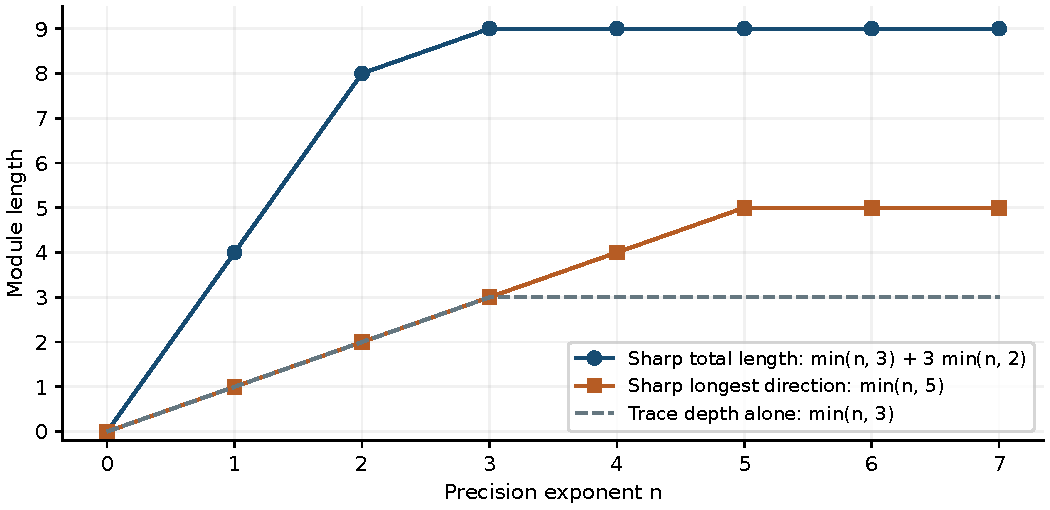
\includegraphics[width=0.94\textwidth]{figures/congruence_lengths.pdf}
 \caption{Exact finite-precision lengths in two extremal rank-two
 families with $a=3$, $e=2$. The first saturates the universal total
 bound; the second saturates the largest-exponent bound $a+e$. The
 curves are values of the proved formulas, not fitted measurements.}
 \label{fig:congruence}
\end{figure}

\subsection{Independent analytic checks}

The program \code{code/verify_grid_projection.py} constructs the averaging
coefficients in two ways: repeated integer convolution and a separate
inclusion--exclusion formula. The run checks 3,318 coefficients exactly,
including positivity, total mass, symmetry and the first two moments.
It also compares the polynomial and exponential multiplier formulas in
160 complex cases at 85-digit working precision and examines 42,000
points of the contraction envelope. The maximum recorded relative
multiplier discrepancy is below $7.5\cdot10^{-85}$.
These numerical comparisons are diagnostics; the inequalities for all
frequencies are proved in Lemma~\ref{grid:lem:contraction}.

\begin{figure}[htbp]
 \centering
 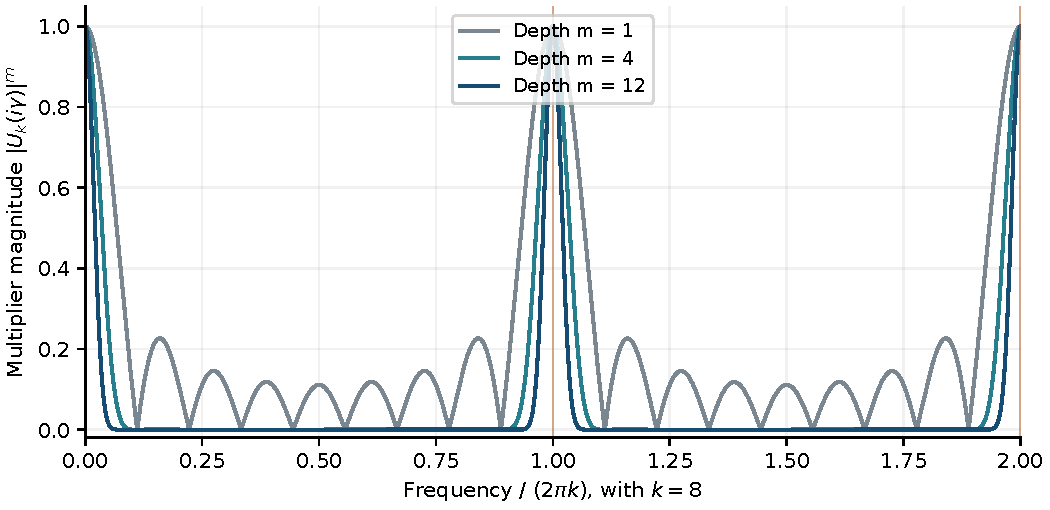
\includegraphics[width=0.94\textwidth]{figures/filter_aliases.pdf}
 \caption{The exact multiplier magnitude $|U_8(i\gamma)|^m$ at three
 depths. Increasing depth damps frequencies away from the lattice
 $2\pi k\mathbb Z$, while every alias remains equal to one. The local
 zero count, not a false uniform damping claim, controls those peaks
 in Theorem~\ref{grid:thm:abstract}.}
 \label{fig:aliases}
\end{figure}

For a direct prime-side illustration the script enumerates 37,128 primes
and 37,308 prime powers through $442{,}413$. It evaluates the identity-class
weight modulo $4$ and the weight $\chi_0+\Re\chi$ for the quartic
character modulo $5$ with $\chi(2)=i$. No zero table or $L$-value routine
is used. With $k=32$, $m=12$, and $t=0$, the values of the normalized
central-order statistic are approximately $0.1862897638670$ and
$0.1727260777212$. These small-depth demonstrations are not certified
central-order determinations and are not asserted to satisfy the
theorem's sufficient rounding threshold. They illustrate the direct
arithmetic computation, including its still-visible decaying remainder.
The complete results are in \code{data/grid_projection_results.json}.

\subsection{What the certificates establish}

The general algebraic theorem is established by its proof, not by a
finite search. The exact computations test its examples and the
implementation of their relation maps. The general analytic theorem is
established by its Fourier estimate and the explicit formula, not by
sampling frequencies. In particular no finite zero computation is used
to infer simplicity, central nonvanishing, or a bound uniform in all
conductors.

Both proofs received a separate internal mathematical review during
preparation. This is distinct from a proof-assistant check or external
peer review. No Lean executable was available in this research
environment, and no new Lean proof is claimed. The file
\code{formalization_outline.md} gives the definitions, intermediate
lemmas and dependency order for a future formalization without embedding
unproved assertions in an apparently completed Lean file.

\subsection{Reproduction and useful next questions}

The archive is self-contained for the new proofs and computations. A
standard LaTeX distribution builds \code{report.tex}; the Python scripts
need SymPy, mpmath, NumPy and Matplotlib, with exact instructions in
\code{README.md}. Upstream repositories are pinned and linked rather
than copied. The provenance files record inspected source hashes,
nearby results and the distinction between classical ingredients and
the proposed new conclusions.

For the algebraic theorem, a finer bound using the entire elementary
divisor profile of each image order could improve specific examples
without changing the sharp universal coefficient. One must still
verify the separate local and automorphic hypotheses before using the
new correction in an enlarged Selmer construction.
For the analytic theorem, worthwhile further work is to instantiate
effective gap and remainder constants for a chosen conductor and to
optimize the finite filter for those constants. The present rate holds
for each fixed family. The synthetic lower bound explains its lattice
alias term but does not establish optimality among all irregular
sampling schedules or among actual Dirichlet zero spectra.

\begin{thebibliography}{99}

\bibitem{Sernau2026}
L. Sernau and collaborators,
\emph{GRH for Dirichlet $L$-functions, in Lean 4},
repository \code{lsernau/grh-lean}, commit
\code{72fead102f663d5c7a407964a13dc0cf9d977207}, 25 November 2026.
\url{https://github.com/lsernau/grh-lean/tree/72fead102f663d5c7a407964a13dc0cf9d977207}.

\bibitem{ProveIt2026}
V. Reshetnikov, \emph{Generalized Riemann Hypothesis: Article},
ProveIt repository, commit
\code{22e5c8b7dda558fd9a50b61465483cb4c0433694}, inspected 27 November 2026.
In particular \code{sections/sel.tex} and \code{sections/ana.tex}.
\url{https://github.com/VladimirReshetnikov/ProveIt/tree/22e5c8b7dda558fd9a50b61465483cb4c0433694/Analysis/GeneralizedRiemannHypothesis/Article}.

\bibitem{Sutherland2026}
A. V. Sutherland,
\emph{Verification files for the shorter Lean proof of RH and of GRH
for Dirichlet $L$-functions}, updated 27 November 2026.
\url{https://math.mit.edu/~drew/shortgrh/}.

\bibitem{Carayol1994}
H. Carayol,
\emph{Formes modulaires et repr\'esentations galoisiennes \`a valeurs
dans un anneau local complet},
Contemporary Mathematics \textbf{165} (1994), 213--237.
\url{https://doi.org/10.1090/conm/165/01601}.

\bibitem{Serre1993}
J.-P. Serre, notes by R. Rouquier,
\emph{Repr\'esentations lin\'eaires sur des anneaux locaux, d'apr\`es
Carayol}, lecture of 8 October 1993, Cours de Jean-Pierre Serre,
volume 14. Theorem 1 is the classical trace-rigidity statement.
\url{https://www.numdam.org/item/CJPS_1993__14_.pdf}.

\bibitem{Brumer2019}
A. Brumer, A. Pacetti, C. Poor, G. Tornar\'ia, J. Voight and D. S. Yuen,
\emph{On the paramodularity of typical abelian surfaces},
Algebra \& Number Theory \textbf{13} (2019), 1145--1195.
\url{https://doi.org/10.2140/ant.2019.13.1145}.
Used as related context for trace-based representation comparison,
not as an input to the new bound.

\bibitem{Hogenauer1981}
E. B. Hogenauer,
\emph{An Economical Class of Digital Filters for Decimation and
Interpolation}, IEEE Transactions on Acoustics, Speech, and Signal
Processing \textbf{29} (1981), no. 2, 155--162.
\url{https://doi.org/10.1109/TASSP.1981.1163535}.
Equation (3) gives the classical cascade polynomial used here.

\bibitem{Bennett2021}
M. A. Bennett, G. Martin, K. O'Bryant and A. Rechnitzer,
\emph{Counting zeros of Dirichlet $L$-functions},
Mathematics of Computation \textbf{90} (2021), 1455--1482.
\url{https://doi.org/10.1090/mcom/3599}.
Author copy:
\url{https://personal.math.ubc.ca/~bennett/BeMaObRe-MathComp-2021.pdf}.

\end{thebibliography}

\end{document}
